\subsection{Diskussion}
\paragraph{symetrische Schwingung}
Es ist wunderbar zu sehen, wie die Eigenschwingung \(\omega_1=\qty{3.89}{\rad\per\s}\) konstant in den Fällen gemessen wird, in denen sie erwartet wird. Im Fall der ungekoppelten Eigenschwingung, dem symetrischen Kopplungsfall, und als FFT des Schwebungsfalls taucht sie auf. Selbstverständlicherweise ist \(\omega_1\not\propto\kappa\). Die fast perfekten Signifkanzen in \cref{table:Vergleichsymasym} unterstreichen diese Erwartung.\\
Leider liegt für den Fall des ungekoppelten Pendels nur eine FFT-Datei vor, deshalb können die Eigenschwingungen der unterschiedlichen Pendel nicht miteinander verglichen werden. Es ist jedoch davon auszugehen, dass durch die Baugleichheit nur eine marginalster Unterschied zu erwarten ist.

\paragraph{asymetrische Schwingung}
Hier ist schön zu sehen, dass \(\omega_2\propto\kappa\). Die Frequenz steigt durch Tiefersetzen des Bronzerings, bei gleicher Pendelamplitude wird der Ring bei tiefere Position dadurch stärker belastet/gedehnt, nach dem Hookschen Gesetz steigt somit die erzeugte Rückstellkraft, die zu einem Steigen von \(\omega_2\) führt. 

\paragraph{Schwebung}
Solange nicht alle Koeffizienten \(A_i,B_i\) aus \cref{eq:allgemeinphi} Null sind, müsste in der Fouriertransformation einer beliebigen gekoppelten Schwingung zumindest eine der beiden Eigenfrequenzen auftauchen. Da die Schwebung gerade durch \(A_1 = -A_2\), \(B_1=B_2=0\) bestimmt ist, besteht die Schwingung letztendlich zum exakt gleichen Anteil aus \(\omega_1\) und \(\omega_2\). Dies ist daran zu sehen, dass in \cref{fig:beat-weakcoupling_fft} der Fouriertransformation beide Gaußpeaks fast gleich hoch sind. \\
Wie gesagt, in \cref{table:Vergleichschwebung} wurden die Eigenschwingungen aus der FFT der Schwebung dargestellt und verglichen, wobei eine sehr gute Übereinstimmung festzustellen ist. In der folgenden \cref{table:Vergleichschwebung} wurden die Cursormessungen benutzt, um die Schwebungsfrequenzen zu bestimmen. In den sehr niedrigen Signifikanzen ist zu sehen, dass die Messergebnisse außergewöhnlich genau sind.

\subsection*{Kopplungsgrade}
Die Ergebnisse beider Untersuchungen (Methodenvergleich: Frequenzen aus sym./asym. FFT vs. aus Schwebungs-FFT, siehe \cref{table:Kopplungsgrade}; als auch Kopplungsgradverhältnisse, siehe \cref{table:Kpplungsgradverhältnisse}) zeigen keine zu hinterfragenden Signifikanzen. Jedoch ist bei \(\kappa^\mathrm{Schwebung}\) schon beobachtbar, dass die Fehler sehr hoch sind, die relativen Fehler liegen bei \(\frac{\Delta\kappa_i}{\kappa_i}=\qtylist{80;40;24}{\percent}\). Bei den Verhältnissen wird dies noch bedrohlicher, die relativen Fehler dieser Werte liegen bei \(\frac{\Delta V^\kappa_i}{V^\kappa_i} =\qtylist{80;86;50}{\percent}\). Keine Ahnung woran diese immensen Fehler liegen.
Die ursprünglichen Fehler der Periodendauern liegen bei \(\Delta T_I/{II}=\qty{}{}\) AH SHIT HERE WE GO AGAIN.
Ich habe natürlich nur die gemessenen Zeiten \(10T,\,7T,\,3T\) durch die Anzahl der Perioden geteilt, nicht aber den Fehler. 
Dafür gibt es diesen Meme:
\xfigure{htbp}{width=\textwidth}{matthew.png}{}{Alles nochmal neu einfügen, wie anstrengend. \autocite{Matthew}}

Hier also nochmal die wichtigen Dinge neu:\par
\begin{table}[htb]
  \centering
  \caption{Vergleich der Schwebungsfrequenzen}
  \begin{tabularx}{\textwidth}{cSZSZZS}
    \toprule
        &{\text{Cursor}}&\text{Superposition}& &\text{Cursor}&\text{Superposition}&\\
        Kopplung&{\(\omega_I[\unit{\rad\per\s}]\)}&\omega_I^\mathrm{beat}[\unit{\rad\per\s}]  &{\(S[\sigma]\)}  &\omega_{II}[\unit{\rad\per\s}] &\omega_{II}^\mathrm{beat}[\unit{\rad\per\s}]&{\(S[\sigma]\)}\\\midrule
        weak&\num{3.97(0.04)}&\num{3.99(0.05)}&\num{0.30}&\num{0.09030(0.00018)}&\num{0.09(0.05)}&\num{0.01}\\
        middle&\num{4.06(0.05)}&\num{4.10(0.09)}&\num{0.40}&\num{0.2051(0.0009)}&\num{0.21(0.09)}&\num{0.05}\\
        strong&\num{4.25(0.13)}&\num{4.27(0.09)}&\num{0.12}&\num{0.370(0.003)}&\num{0.37(0.09)}&\num{0.05}\\
        \bottomrule
  \end{tabularx}
\label{table:Vergleichschwebungneu}  
\end{table} 
Man sieht jetzt also sehr schön, dass der Fehler für \(\omega_I\) deutlich kleiner geworden ist, gegenüber der ersten Lösung. Auch steigt der Fehler \(\Delta \omega_I\) mit höherer Kopplung, da wir hier immer weniger Perioden gemessen haben, das heißt \(\frac{\Delta T_I}{T_I}\) wird größer. Dies ist die schnelle/innere Frequenz der Schwebung, deren Fehler vorhin zu groß war (pauschal auf \(\qty{0.14}{\s}\) gesetzt, obwohl über mehrere Perioden gemessen wurde). \(\Delta T=\sqrt{2}\cdot\qty{0.1}{\s}\) kommt übrigens daher, dass wir mit dem Cursor auf beiden Seiten (Startzeit \verb|T_1|-Endzeit \verb|T_2| in \cref{fig:redactet} ) jeweils um \(\qty{0.1}{\s}\) genau messen konnten.  
\newpage
\begin{table}[htb]
  \centering
  \caption{Kopplungsgrade, einmal bestimmt über \(\omega_{1/2}\) (sym./asym.) und einmal über \(T_{I/II}\)(Schwebung)}
  \begin{tabularx}{\textwidth}{TZZZ}
    \toprule
        Kopplung& \kappa^\mathrm{sym./asym.} & \kappa^\mathrm{Schwebung} & S[\sigma]\\\midrule
        weak&\num{0.05(0.04)}&\num{0.0454(0.0004)}&\num{0.7}\\
        middle&\num{0.10(0.04)}&\num{0.1007(0.0014)}&\num{0.9}\\
        strong&\num{0.17(0.04)}&\num{0.173(0.006)}&\num{1.0}\\
    \bottomrule
  \end{tabularx}
\label{table:Kopplungsgradeneu}  
\end{table} 
Anhand dieser neuen Ergebnisse beobachtet man sehr schön, dass die relativen Fehler der Kopplungsgrade deutlich kleiner geworden sind. 

\begin{table}[htb]
  \centering
  \caption{Verhältnisse der Kopplungsgrade}
  \begin{tabularx}{\textwidth}{ZZZZ}
    \toprule
        \text{Kopplung}& V^l & V^\kappa & S[\sigma]\\\midrule
        \nicefrac{\kappa_w}{\kappa_m}&\num{0.432(0.005)}&\num{0.451(0.007)}&\num{0.9}\\
        \nicefrac{\kappa_w}{\kappa_s}&\num{0.240(0.003)}&\num{0.262(0.009)}&\num{0.9}\\
        \nicefrac{\kappa_m}{\kappa_s}&\num{0.555(0.005)}&\num{0.582(0.022)}&\num{0.9}\\
    \bottomrule
  \end{tabularx}
\label{table:Kpplungsgradverhältnisseneu}  
\end{table} 
Wiederum dasselbe wie oben schon, die relativen Fehler sind auf ein angenehmes Niveau gesunken.

\subsection{Fouriertransformationfehler}
Was in \cref{table:Vergleichsymasym} schon zu sehen ist: die erste Zeile (weak) hat den kleinsten Fehler für \(\omega_{I/II}\), da hier die längste Zeitspanne aufgenommen wurde. Somit ist die Fouriertransformation genauer und die FHWM der Peaks kleiner. \\
Was den Effekt durch Reibung angeht, den man in \cref{fig:assymetricweakcoupling} sieht, so sollte meiner naiven Sichtweise nach dies eine Auswirkung haben: Denn die Fouriertransformation
\begin{equation}
    X(f)=\int_{0}^{T}x(t)e^{-i2\pi ft}\diff t
\end{equation}
bzw. für zeitdiskrete Signale von N-Messpunkten:
\begin{equation}
    X(f)=\sum_{t=0}^{N-1}x(t)e^{-i2\pi \cdot \frac{tf}{N}}\quad t\in(0,N-1)
\end{equation}
ist abhängig von der Amplitude \(x(t)\) im Ortsraum, die durch Reibung sinkt. Wie genau die mathematische Auswirkung ist, weiß ich nicht.
\par
Zusätzlich sieht man in \cref{fig:assymetricweakcoupling} sehr schön den im Skript angesprochenen Effekt, dass symetrische und assymetrische Schwingung nicht exakt angeregt werden können - eine leichte Schwebung ist zu sehen.\par
In der Zusatzdatei \autocite{Dimitrij} ist ein interessanter Code bereitgestellt, mit dem man genau obige zeitdiskrete Fouriertransformation für eine bestimmte Anzahl an Messwerten (Anzahl ist natürlich abhängig von der Messdauer \(T\) und Abtastrate der \(x(t)\) Amplitude) anhand der Funktion der symetrischen Schwingung \(f=\varphi_0\cos(\omega_1t)\) durchführen kann. Hierzu wird das einstellbare Messintervall \(T\) auf verschiedene Dauern eingestellt, um den Effekt auf die Fouriertransformation \(\mathcal{F}[f(t)](\omega)\) zu untersuchen. Wie erwartet und vorhin erwähnt, ergeben sich für eine längere Aufnahmezeit schärfere Peaks im Fourierraum, sodass die der Schwingung zugrundeliegende Frequenz genauer extrahiert werden kann. Dies liegt daran, dass eine verringerte Messdauer damit einhergeht, dass mit der \(x(t)\) eine Rechteckfunktion der Breite \(T\) multipliziert wird. Deren Fouriertrafo ist die sinc-Funktion, die für unendliche Zeiten \(T\) im distributionellen Sinne in die Delta-Distribution übergeht\autocite{sincfunction}.
\begin{gather*}
  \mathcal{F}[\mathrm{rect\left(\frac{t}{T}\right)}](\omega)=\int_{0}^{T}e^{-i\omega t} \diff t= T\,\operatorname{sinc}\left(\frac{\omega T}{2}\right)\\
  \lim_{T\to\infty}T\,\operatorname{sinc}\left(\frac{\omega T}{2}\right)=\delta(\omega)
\end{gather*}
\xfigure{htbp}{width=0.7\textwidth}{Fouriertrafos.png}{}{Betrachtung der Auswirkung der Messdauer auf die Schärfe der Fouriertransformation}

Ich hab noch die FHWM ausgerechnet, und man sieht wunderbar komplementäre Resultate: Bei der symetrischen Schwingung haben wir eine Aufnahmedauer von \(T=\qty{60}{\s}\) gehabt (in der \verb|.tx(t)| Datei nachgeschaut). Hier ware die vom dortigen Python-Programm anhand der realen Amplitudenwerte ausgerechnete FHWM \(\qty{0.12}{\rad\per\s}\). Ich meine, es sollte zum Python-Skript (\jump{page.28}{\texttt{.iynb}-Datei, Seite 9}), aus dem \cref{fig:Fouriertrafos.png} entstanden ist, kein Unterschied zu erkennen sein, denn hier wurde ja genau die Funktion der symetrischen Schwingung transformiert, die im Labor vermessen wurde (bis auf einen anderen Auslenkwinkel). Es ergibt sich auch eine FHWM von \(\qty{0.12}{\rad\per\s}\).
\vspace{3cm}
\begin{wrapfigure}{r}{0.4\textwidth}
    
\includegraphics[height=0.6\textheight]{fookinspacecharacters.png}
    \caption{Die Einstellung auf weak,\dots\;hatte einen einzigen Sinn smh. \autocite{Thatcher}}
\end{wrapfigure}
\subsection{Fazit}
Schöner Versuch, Auswertung an sich war sehr angenehm, und nicht so ewig. Hab aber trotzdem für alles drumrum zu lange gebraucht (die Memes und Minecraft sind schuld).\\
Ich hab keine Ahnung, woran es liegt, aber ich kann die ganzen SVG mit Inkscape nicht als \verb|.pdf| exportieren, als \verb|.png| war mir zu langweilig. Ich hab ewig versucht, das \tcboxverb[colback=blueurllink!40!white]{svg} Package zu benutzen, aber bin aus der \href{https://mirror.funkfreundelandshut.de/latex/graphics/svg/doc/svg.pdf}{Documentation} nicht schlau geworden, ob man durch \verb|\includeinkscape| auch ohne \verb|--shell-escape| arbeiten kann. Auf jeden Fall hat der \verb|.pdf_tex| Export über Inkscape auch nicht funktioniert. Wenigstens will ich noch hiermit über die Benennung der Dateien ranten:
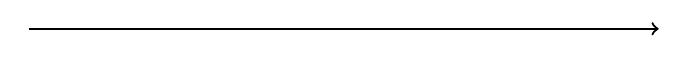
\begin{tikzpicture}
  \draw[thick,->](0,2)--(8,2);
\end{tikzpicture}

% \xfigure{htbp}{height=0.5\textheight}{fookinspacecharacters.png}{}{Die Einstellung auf weak,\dots hatte einen einzigen Sinn smh. \autocite{Thatcher}}
